% CS6140 Homework Assignment Template
% Computer Science
% Northeastern University
% Boston, MA 02115

% Do not manipulate any of the settings
\documentclass[twoside]{article}

\usepackage{epsfig}
\usepackage{natbib}
\usepackage{units}
\usepackage{amssymb}
\usepackage{amsmath}
\usepackage{babel}


\setlength{\oddsidemargin}{0 in}
\setlength{\evensidemargin}{0 in}
\setlength{\topmargin}{-0.6 in}
\setlength{\textwidth}{6.5 in}
\setlength{\textheight}{8.5 in}
\setlength{\headsep}{0.75 in}
\setlength{\parindent}{0 in}
\setlength{\parskip}{0.1 in}

\newcommand{\lecture}[3]{
   \pagestyle{myheadings}
   \thispagestyle{plain}
   \newpage
   \setcounter{page}{1}
   \noindent
   \begin{center}
   \framebox{
      \vbox{\vspace{2mm}
    \hbox to 6.28in { {\bf CS6140: Machine Learning\hfill} }
       \vspace{6mm}
       \hbox to 6.28in { {\Large \hfill #1  \hfill} }
       \vspace{6mm}
       \hbox to 6.28in { {\it Assigned: #2 \hfill Due: #3} }
      \vspace{2mm}}
   }
   \end{center}
   \markboth{#1}{#1}
   \vspace*{4mm}
}

\begin{document}

% to have alphanumeric enumeration (Hasan's command)
\renewcommand{\labelenumi}{\alph{enumi})}

\lecture{Homework Assignment \# 2}{02/05/2020}{02/18/2020, 11:59pm, through Blackboard}

\begin{center}
Name: Piyush Goel\\
Email: goel.pi@husky.neu.edu
\end{center}

%%
%% Problem
%%

\textbf{Problem 1.} (25 points) Naive Bayes classifier. Consider a binary classification problem where there are only four data points in the training set. That is $\mathcal{D}=\left\{ (-1,-1,-),(-1,+1,+),(+1,-1,+),(+1,+1,-)\right\} $, where each tuple $(x_{1},x_{2},y)$ represents a training example with input vector $(x_{1},x_{2})$ and class label $y$.

\begin{enumerate}
\item (10 points) Construct a naive Bayes classifier for this problem and evaluate its accuracy on the training set. Consider ``accuracy'' to be the fraction of correct predictions.
\item (10 points) Transform the input space into a six-dimensional space $(+1, x_{1}, x_{2}, x_{1}x_{2}, x_{1}^{2}, x_{2}^{2})$ and repeat the previous step.
\item (5 points) Repeat the previous step when the data set accidentally includes the seventh feature, set to $-x_{1}x_{2}$. What is the impact of adding this dependent feature on the classification model?
\end{enumerate}
Carry out all steps manually and show all your calculations.


\textbf{Solution}
\begin{enumerate}
    \item 
    The prior probabilities are as follows: $p(+) = 1/2, p(-) = 1/2$\\
    Likelyhood of the feature $x_1$: $p(x_1 = 1|+) = p(x_1=-1|+) = p(x_1=1|-) = p(x_1=-1|-) = 1/2$\\
    Likelyhood of the feature $x_2$: $p(x_2 = 1|+) = p(x_2=-1|+) = p(x_2=1|-) = p(x_2=-1|-) = 1/2$
    Posterior probabilities:\\
    \begin{equation*}
        p(+|X_1) = \frac{p(X_1|+)p(+)}{p(X_1|+)p(+) + p(X_1|-)p(-)} = \frac{p(x_1=-1, x_2=-1|+)p(+)}{p(x_1=-1, x_2=-1|+)p(+) + p(x_1=-1, x_2=-1|-)p(-)}
    \end{equation*}
    Now, using the Naive Bayes' assumption.
    \begin{equation*}
        p(+|X_1) = \frac{p(x_1=-1|+)p(x_2=-1|+)p(+)}{p(x_1=-1|+)p(x_2=-1|+)p(+) + p(x_1=-1|-)p(x_2=-1|-)p(-)} = 1/2
    \end{equation*}
    Similarly,
    \begin{equation*}
        p(-|X_1) = \frac{p(x_1=-1|-)p(x_2=-1|-)p(-)}{p(x_1=-1|+)p(x_2=-1|+)p(+) + p(x_1=-1|-)p(x_2=-1|-)p(-)} = 1/2
    \end{equation*}
    \begin{equation*}
        p(+|X_2) = \frac{p(x_1=-1|+)p(x_2=1|+)p(+)}{p(x_1=-1|+)p(x_2=1|+)p(+) + p(x_1=-1|-)p(x_2=1|-)p(-)} = 1/2
    \end{equation*}
    \begin{equation*}
        p(-|X_2) = \frac{p(x_1=-1|-)p(x_2=1|-)p(-)}{p(x_1=-1|+)p(x_2=1|+)p(+) + p(x_1=-1|-)p(x_2=1|-)p(-)} = 1/2
    \end{equation*}
    \begin{equation*}
        p(+|X_3) = \frac{p(x_1=1|+)p(x_2=-1|+)p(+)}{p(x_1=1|+)p(x_2=-1|+)p(+) + p(x_1=1|-)p(x_2=-1|-)p(-)} = 1/2
    \end{equation*}
    \begin{equation*}
        p(-|X_3) = \frac{p(x_1=1|-)p(x_2=-1|-)p(-)}{p(x_1=1|+)p(x_2=-1|+)p(+) + p(x_1=1|-)p(x_2=-1|-)p(-)} = 1/2
    \end{equation*}
        \begin{equation*}
        p(+|X_4) = \frac{p(x_1=1|+)p(x_2=1|+)p(+)}{p(x_1=1|+)p(x_2=1|+)p(+) + p(x_1=1|-)p(x_2=1|-)p(-)} = 1/2
    \end{equation*}
    \begin{equation*}
        p(-|X_4) = \frac{p(x_1=1|-)p(x_2=1|-)p(-)}{p(x_1=1|+)p(x_2=1|+)p(+) + p(x_1=1|-)p(x_2=1|-)p(-)} = 1/2
    \end{equation*}
    Since, this classifier classifies both the correct outcomes and the incorrect outcomes with the probability of $0.5$, therefore the accuracy of the classifier can be said to be as $0.5$ (or 50\%).
    
    \item
    The posterior probabilities and the likelyhoods of the old features would remain the same from the previous part. Likelyhoods of the new features:
    \begin{equation*}
        p(+1|+) = 1/2, p(+1|-) = 1/2,
    \end{equation*}
    \begin{equation*}
        p(x_1x_2 = 1|+) = 0, p(x_1x_2 = -1|+) = 1, p(x_1x_2 = 1|-) = 1, p(x_1x_2 = -1|-) = 0,
    \end{equation*}
    \begin{equation*}
        p(x_1^2 = 1|+) = 1, p(x_1^2 = -1|+) = 0, p(x_1^2 = 1|-) = 1, p(x_1^2 = -1|-) = 0,
    \end{equation*}
        \begin{equation*}
        p(x_2^2 = 1|+) = 1, p(x_2^2 = -1|+) = 0, p(x_2^2 = 1|-) = 1, p(x_2^2 = -1|-) = 0.
    \end{equation*}
    
    Using the Naive Bayes' Assumption:
    \begin{equation*}
        p(X_1|+) = p(+1|+)p(x_1=-1|+)p(x_2=-1|+)p(x_1x_2=1|+)p(x_1^2=1|+)p(x_2^2=1|+) = 0
    \end{equation*}
    Therefore, $p(+|X_1) = 0$ and $p(-|X_1) = 1$
    Similarly, we get
    \begin{equation*}
         p(X_2|+) = p(+1|+)p(x_1=-1|+)p(x_2=1|+)p(x_1x_2=-1|+)p(x_1^2=1|+)p(x_2^2=1|+) = 1/8
    \end{equation*}
    Therefore, $p(+|X_2) = 1$ and $p(-|X_2) = 0$.
    Similarly,
    \begin{equation*}
        p(X_3|+) = p(+1|+)p(x_1=1|+)p(x_2=-1|+)p(x_1x_2=-1|+)p(x_1^2=1|+)p(x_2^2=1|+) = 1/8
    \end{equation*}
    Therefore, $p(+|X_3) = 1$ and $p(-|X_3) = 0$.
    Similarly,
    \begin{equation*}
        p(X_4|+) = p(+1|+)p(x_1=1|+)p(x_2=1|+)p(x_1x_2=1|+)p(x_1^2=1|+)p(x_2^2=1|+) = 0
    \end{equation*}
    Therefore, $p(+|X_4) = 0$ and $p(-|X_4) = 1$.\\
    This classifier makes the correct guess in each case therefore its accuracy is $1$ (or 100\%).
    
    \item
    The posterior probabilities and the likelyhoods of the old features would remain the same from the previous part. Likelyhoods of the new features:
    \begin{equation*}
        p(-x_1x_2 = 1|+) = 1, p(-x_1x_2 = -1|+) = 0, p(-x_1x_2 = 1|-) = 0, p(-x_1x_2 = -1|-) = 1
    \end{equation*}
     Its likelyhood would always have the same value as the likelyhood of the feature $x_1x_2$, and since that likelyhood is always either 1 or 0, adding this extra feature would not change any of the likelyhoods or the posterior probabilities as shown below:
    \begin{equation*}
        p(X_1|+) = p(+1|+)p(x_1=-1|+)p(x_2=-1|+)p(x_1x_2=1|+)p(x_1^2=1|+)p(x_2^2=1|+)p(-x_1x_2=-1|+) = 0
    \end{equation*}
    \begin{equation*}
        p(X_2|+) = p(+1|+)p(x_1=-1|+)p(x_2=1|+)p(x_1x_2=-1|+)p(x_1^2=1|+)p(x_2^2=1|+)p(-x_1x_2 = 1|+) = 1/8
    \end{equation*}
    \begin{equation*}
        p(X_3|+) = p(+1|+)p(x_1=1|+)p(x_2=-1|+)p(x_1x_2=-1|+)p(x_1^2=1|+)p(x_2^2=1|+)p(-x_1x_2 = 1|+) = 1/8
    \end{equation*}
    \begin{equation*}
        p(X_4|+) = p(+1|+)p(x_1=1|+)p(x_2=1|+)p(x_1x_2=1|+)p(x_1^2=1|+)p(x_2^2=1|+)p(-x_1x_2=-1|+) = 0
    \end{equation*}
    Hence, $p(+|X_1) = 0 , p(-|X_1) = 1 , p(+|X_2) = 1 , p(-|X_2) = 0 , p(+|X_3) = 1 , p(-|X_3) = 0 , p(+|X_4) = 0 , p(-|X_4) = 1$. And as we can see all these probabilities remain the same as the previous part.\\
    Therefore the accuracy of this classifier is 1 (or 100\%) as well.
\end{enumerate}


%%
%% Problem
%%

\textbf{Problem 2.} (25 points) Consider a binary classification problem in which we want to determine the optimal decision surface. A point $\mathbf{x}$ is on the decision surface if $P(Y=1|\mathbf{x})=P(Y=0|\mathbf{x})$.

\begin{enumerate}
\item (10 points) Find the optimal decision surface assuming that each class-conditional distribution is defined as a two-dimensional Gaussian distribution:
\[
p(\mathbf{x}|Y=i)=\frac{1}{(2\pi)^{\nicefrac{d}{2}} |\mathbf{\Sigma}_{i}|^{\nicefrac{1}{2}}}\cdot e^{-\frac{1}{2}(\mathbf{x}-\mathbf{m}_{i})^{T}\mathbf{\Sigma}_{i}^{-1}(\mathbf{x}-\mathbf{m}_{i})}
\]
where $i \in \left\{ 0, 1\right\}$, $\mathbf{m}_{0}=(1,2)$, $\mathbf{m}_{1}=(6,3)$, $\mathbf{\Sigma}_{0}=\mathbf{\Sigma}_{1}=\mathbf{I}_2$, $P(Y=0)=P(Y=1)=\nicefrac{1}{2}$, $\mathbf{I}_d$ is the $d$-dimensional identity matrix, and $|\mathbf{\Sigma}_{i}|$ is the determinant of $\mathbf{\Sigma}_{i}$.
\item (5 points) Generalize the solution from part (a) using $\mathbf{m}_{0}=(m_{01}, m_{02})$, $\mathbf{m}_{1}=(m_{11}, m_{12})$, $\mathbf{\Sigma}_{0}=\mathbf{\Sigma}_{1}=\sigma^2 \mathbf{I}_2$ and $P(Y=0)\neq P(Y=1)$.
\item (10 points) Generalize the solution from part (b) to arbitrary covariance matrices $\mathbf{\Sigma}_{0}$ and $\mathbf{\Sigma}_{1}$. Discuss the shape of the optimal decision surface.
\end{enumerate}


\textbf{Solution}
\begin{enumerate}
	\item
	We know that the boundary of the decision surface can be calculated by $P(Y=1|\mathbf{x})=P(Y=0|\mathbf{x})$.
	Therefore, we get
	\begin{equation*}
		\frac{p(\mathbf{x}|Y=1)P(Y=1)}{p(\mathbf{x})} = \frac{p(\mathbf{x}|Y=1)P(Y=0)}{p(\mathbf{x})}
	\end{equation*}
	Therefore,
	\begin{equation*}
		p(\mathbf{x}|Y=1) = p(\mathbf{x}|Y=0)
	\end{equation*}
	\begin{equation*}
		\frac{1}{(2\pi)^{\nicefrac{1}{2}} |\mathbf{\Sigma}_{1}|^{\nicefrac{1}{2}}}\cdot e^{-\frac{1}{2}(\mathbf{x}-\mathbf{m}_{1})^{T}\mathbf{\Sigma}_{1}^{-1}(\mathbf{x}-\mathbf{m}_{1})} = \frac{1}{(2\pi)^{\nicefrac{1}{2}} |\mathbf{\Sigma}_{2}|^{\nicefrac{1}{2}}}\cdot e^{-\frac{1}{2}(\mathbf{x}-\mathbf{m}_{2})^{T}\mathbf{\Sigma}_{2}^{-1}(\mathbf{x}-\mathbf{m}_{2})}
	\end{equation*}
	Canceling the constants on both sides since they're the same and then taking log of both sides (we can do this because both sides are positive), we get
	\begin{equation*}
		(\mathbf{x}-\mathbf{m}_{1})^{T}\mathbf{\Sigma}_{1}^{-1}(\mathbf{x}-\mathbf{m}_{1}) = (\mathbf{x}-\mathbf{m}_{2})^{T}\mathbf{\Sigma}_{2}^{-1}(\mathbf{x}-\mathbf{m}_{2})
	\end{equation*}
	Taking $\mathbf{x} = \begin{bmatrix} x_1 & x_2 \end{bmatrix}$ and taking the values of all the other matrices we get,
	\begin{equation*}
		(x_1 - 1)^2 + (x_2 - 2)^2 = (x_1 - 6)^2 + (x_2 - 3)^2
	\end{equation*}
	\begin{equation*}
		5x_1 + x_2 = 20
	\end{equation*}
	
	
	\item
	We know that the boundary of the decision surface can be calculated by $P(Y=1|\mathbf{x})=P(Y=0|\mathbf{x})$.
	Therefore, we get
	\begin{equation*}
		\frac{p(\mathbf{x}|Y=1)P(Y=1)}{p(\mathbf{x})} = \frac{p(\mathbf{x}|Y=1)P(Y=0)}{p(\mathbf{x})}
	\end{equation*}
	Taking $P(Y=1) = p$ and $P(Y=0) = 1 - p$. Therefore,
	\begin{equation*}
		p\frac{1}{(2\pi)^{\nicefrac{1}{2}} |\mathbf{\Sigma}_{1}|^{\nicefrac{1}{2}}}\cdot e^{-\frac{1}{2}(\mathbf{x}-\mathbf{m}_{1})^{T}\mathbf{\Sigma}_{1}^{-1}(\mathbf{x}-\mathbf{m}_{1})} = (1-p)\frac{1}{(2\pi)^{\nicefrac{1}{2}} |\mathbf{\Sigma}_{2}|^{\nicefrac{1}{2}}}\cdot e^{-\frac{1}{2}(\mathbf{x}-\mathbf{m}_{2})^{T}\mathbf{\Sigma}_{2}^{-1}(\mathbf{x}-\mathbf{m}_{2})}
	\end{equation*}
	Canceling common constants and taking log of both sides, we get
	\begin{equation*}
	(-1/2)(\mathbf{x}-\mathbf{m}_{1})^{T}\mathbf{\Sigma}_{1}^{-1}(\mathbf{x}-\mathbf{m}_{1}) + \log p= (-1/2)(\mathbf{x}-\mathbf{m}_{2})^{T}\mathbf{\Sigma}_{2}^{-1}(\mathbf{x}-\mathbf{m}_{2}) + \log 1 - p
	\end{equation*}
	Taking $\mathbf{x} = \begin{bmatrix} x_1 & x_2 \end{bmatrix}$ and taking the values of all the other matrices we get,
	\begin{equation*}
		\frac{(x_1-m_{01})^2 + (x_2 - m_{02})^2}{2\sigma^2} + \log p = \frac{(x_1-m_{11})^2 + (x_2 - m_{12})^2}{2\sigma^2} + \log 1-p 
	\end{equation*}
	\begin{equation*}
		x_1^2-2x_1m_{01}+m_{01}^2 + x_2^2 -2x_2m_{02} + m_{02}^2 + 2\sigma^2\log p = x_1^2-2x_1m_{11}+m_{11}^2 + x_2^2 -2x_2m_{12} + m_{12}^2 + 2\sigma^2\log 1-p 
	\end{equation*}
	Therefore we get the equation of the decision surface as
	\begin{equation*}
		2x_1(m_{11}-m_{01}) + 2x_2(m_{12} - m_{02}) + m_{01}^2 + m_{02}^2 - m_{11}^2 - m_{12}^2 + 2\sigma^2\log\frac{p}{1-p} = 0
	\end{equation*}
	
	\item
	We know that the boundary of the decision surface can be calculated by $P(Y=1|\mathbf{x})=P(Y=0|\mathbf{x})$.
	Therefore, we get
	\begin{equation*}
		\frac{p(\mathbf{x}|Y=1)P(Y=1)}{p(\mathbf{x})} = \frac{p(\mathbf{x}|Y=1)P(Y=0)}{p(\mathbf{x})}
	\end{equation*}
	Taking $P(Y=1) = p$ and $P(Y=0) = 1 - p$. Therefore,
	\begin{equation*}
		p\frac{1}{(2\pi)^{\nicefrac{1}{2}} |\mathbf{\Sigma}_{1}|^{\nicefrac{1}{2}}}\cdot e^{-\frac{1}{2}(\mathbf{x}-\mathbf{m}_{1})^{T}\mathbf{\Sigma}_{1}^{-1}(\mathbf{x}-\mathbf{m}_{1})} = (1-p)\frac{1}{(2\pi)^{\nicefrac{1}{2}} |\mathbf{\Sigma}_{2}|^{\nicefrac{1}{2}}}\cdot e^{-\frac{1}{2}(\mathbf{x}-\mathbf{m}_{2})^{T}\mathbf{\Sigma}_{2}^{-1}(\mathbf{x}-\mathbf{m}_{2})}
	\end{equation*}
	Canceling common constants and taking log of both sides, we get the equation of the decision boundary in vector form as follows
	\begin{equation*}
		(-1/2)(\mathbf{x}-\mathbf{m}_{1})^{T}\mathbf{\Sigma}_{1}^{-1}(\mathbf{x}-\mathbf{m}_{1}) + \log p -(1/2)\log|\mathbf{\Sigma}_1|= (-1/2)(\mathbf{x}-\mathbf{m}_{2})^{T}\mathbf{\Sigma}_{2}^{-1}(\mathbf{x}-\mathbf{m}_{2}) + \log (1 - p) -(1/2)\log|\mathbf{\Sigma}_2|
	\end{equation*}
	Simplifying it further we get
	\begin{equation*}
		\mathbf{x}^T(\mathbf{\Sigma}_1^{-1} - \mathbf{\Sigma}_2^{-1})\mathbf{x} - (\mathbf{m}_{1}^T\mathbf{\Sigma}_1^{-1} - \mathbf{m}_{2}^T\mathbf{\Sigma}_2^{-1})\mathbf{x} - \mathbf{x}^T(\mathbf{\Sigma}_1^{-1}\mathbf{m}_{1} - \mathbf{\Sigma}_2^{-1}\mathbf{m}_{2}) + \mathbf{m}_{1}\mathbf{\Sigma}_1^{-1}\mathbf{m}_{1}^T - \mathbf{m}_{2}\mathbf{\Sigma}_2^{-1}\mathbf{m}_{2}^T -2\log \frac{p}{1-p} + \log\frac{|\mathbf{\Sigma}_1|}{|\mathbf{\Sigma}_2|} = 0
	\end{equation*}
	In both of the previous parts the decision surface was just a linear plane of d-dimensions (2 in those cases) because its equation was just the linear combination of all the features (i.e. $x_1$ and $x_2$). In this part though, the equation of the decision surface is not just a linear combination but rather terms of degree 2 may exist as well. Hence the surface will be a \textbf{quadratic plane}. Though this would depend on the value of the covariance matrices, if $\Sigma_1 = \Sigma_2$, then the coefficient of the quadratic term would be zero and hence the equation of the plane would only contain linear terms in $x$, and would result in a linear plane in the d-dimensions.

\end{enumerate}



%%
%% Problem
%%

\textbf{Problem 3.} (45 points) Consider a multivariate linear regression problem of mapping $\mathbb{R}^d$ to $\mathbb{R}$, with two different objective functions. The first objective function is the sum of squared errors, as presented in class; i.e., $\sum_{i=1}^{n}e_{i}^2$, where $e_i=w_0 + \sum_{j=1}^{d}w_jx_{ij} - y_i$. The second objective function is the sum of square Euclidean distances to the hyperplane; i.e., $\sum_{i=1}^{n}r_{i}^2$, where $r_i$ is the Euclidean distance between point $(x_i,y_i)$ to the hyperplane $f(x)=w_0 + \sum_{j=1}^{d}w_jx_j$.

\begin{enumerate}
\item (5 points) Derive a gradient descent algorithm to find the parameters of the model that minimizes the sum of squared errors. 

\item (20 points) Derive a gradient descent algorithm to find the parameters of the model that minimizes the sum of squared distances. 

\item (20 points) Implement both algorithms and test them on 5 datasets. Datasets can be randomly generated, as in class, or obtained from resources such as UCI Machine Learning Repository. Compare the solutions to the closed-form (maximum likelihood) solution derived in class and find the $R^2$ in all cases on the same dataset used to fit the parameters; i.e., do not implement cross-validation.
\end{enumerate}


\textbf{Solution}
\begin{enumerate}
    \item 
    The objective function:
    \begin{equation*}
        C = \sum_{i=1}^n e_i^2 = \sum_{i=1}^n \left(w_0 + \sum_{j=1}^d w_j x_{ij} - y_i\right)^2
    \end{equation*}
    The partial derivative of the objective function with respect to some $w_k \forall k \in [1,d]$:
    \begin{equation*}
        \frac{\partial C}{\partial w_k} = 2\sum_{i=1}^n \left(w_0 + \sum_{j=1}^d w_j x_{ij} - y_i\right)x_{ik}
    \end{equation*}
    The partial derivative of the objective function with respect to $w_0$ is:
    \begin{equation*}
		\frac{\partial C}{\partial w_0} = 2\sum_{i=1}^n \left(w_0 + \sum_{j=1}^d w_j x_{ij} - y_i\right)
	\end{equation*}

    Let $W = \begin{bmatrix} w_0\\w_1\\ \vdots\\ w_d \end{bmatrix}$ and $\Delta = \begin{bmatrix} \frac{\partial C}{\partial w_0}\\\frac{\partial C}{\partial w_1}\\ \vdots\\ \frac{\partial C}{\partial w_1} \end{bmatrix}$.\\
    Therefore the gradient descent update becomes: $W^{(t+1)} = W^{(t)} - \eta \Delta ^ {(t)}$.Now, we just have to initialize the value of $W^{(0)}$ and choose an appropriate $\eta$, then we can just run the update until convergence, and this is the gradient descent algorithm.
    
    \item
    The objective function:
    \begin{equation*}
        C = \sum_{i = 1}^n r_i^2 = \sum_{i = 1}^n \left( \frac{w_0 + \sum_{j = 1}^d w_j x_{ij} - y_i}{\sqrt{1 + \sum_{j=1}^d w_j^2}} \right)^2
    \end{equation*}
    The partial derivative of the objective function with respect to some $w_k \forall k \in [1,d]$:
    \begin{equation*}
        \frac{\partial C}{\partial w_k} =  \sum_{i = 1}^n \frac{2(w_0 + \sum_{j=1}^d w_j x_{ij} -y_i)x_{ik}(1 + \sum_{j=1}^d w_j^2) - 2w_k(w_0 + \sum_{j=1}^d w_j x_{ij} -y_i)^2}{(1 + \sum_{j=1}^d w_j^2)^2}
    \end{equation*}
    \begin{equation*}
    	\frac{\partial C}{\partial w_k} =  2\sum_{i = 1}^n \frac{(w_0 + \sum_{j=1}^d w_j x_{ij} -y_i)\left(x_{ik}(1 + \sum_{j=1}^d w_j^2) - w_k(w_0 + \sum_{j=1}^d w_j x_{ij} -y_i)\right)}{(1 + \sum_{j=1}^d w_j^2)^2}
    \end{equation*}
    The partial derivative of the objective function with respect to $w_0$:
    \begin{equation*}
    	\frac{\partial C}{\partial w_0} = 2\sum_{i = 1}^n \frac{(w_0 + \sum_{j=1}^d w_j x_{ij} -y_i)}{(1 + \sum_{j=1}^d w_j^2)}
    \end{equation*}
    Let $W = \begin{bmatrix} w_0\\w_1\\ \vdots\\ w_d \end{bmatrix}$ and $\Delta = \begin{bmatrix} \frac{\partial C}{\partial w_0}\\\frac{\partial C}{\partial w_1}\\ \vdots\\ \frac{\partial C}{\partial w_1} \end{bmatrix}$.\\
    Therefore the gradient descent update becomes: $W^{(t+1)} = W^{(t)} - \eta \Delta ^ {(t)}$.Now, we just have to initialize the value of $W^{(0)}$ and choose an appropriate $\eta$, then we can just run the update until convergence, and this is the gradient descent algorithm.
    
    \item
%	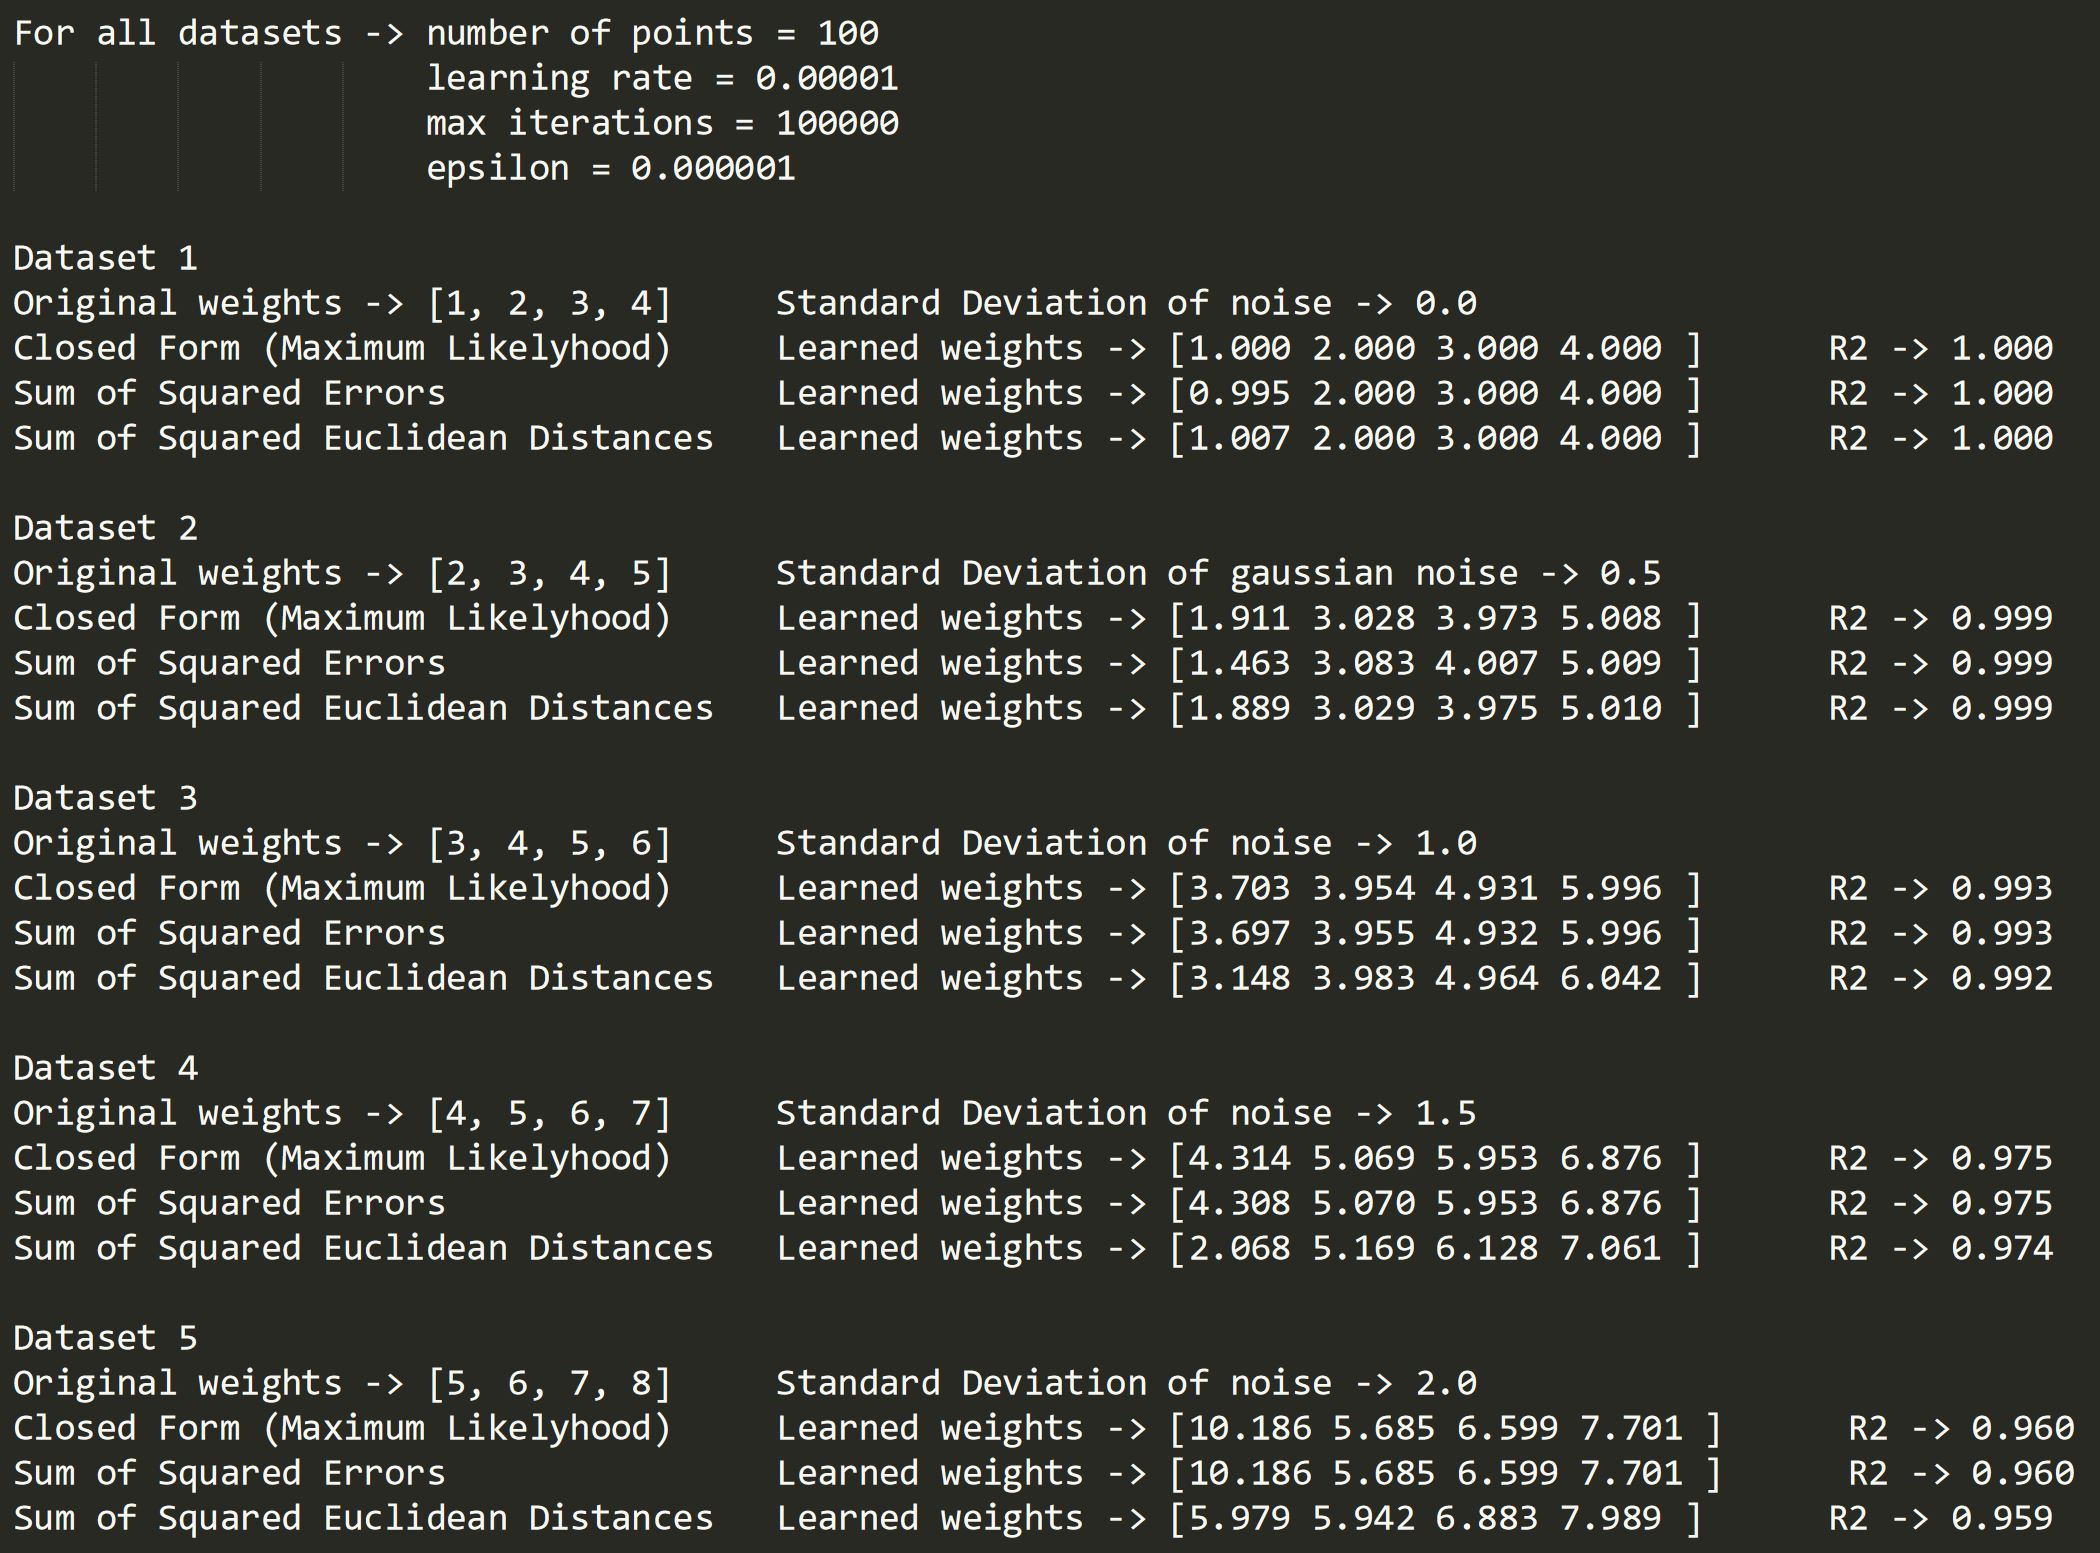
\includegraphics[scale=0.7]{prob3_output}
    
\end{enumerate}



\end{document}